\documentclass[10pt,a4paper,oneside]{beamer}
\usepackage[utf8]{inputenc}
\usepackage{amsmath}
\usepackage{amsfonts}
\usepackage{amssymb}
\usepackage{graphicx}
\usepackage{breqn}
\usepackage{tikz} % system block diagram
\usepackage{textcomp}
\usetikzlibrary{shapes,arrows} % system block diagram
\usepackage{booktabs}
\usepackage[framed,numbered,autolinebreaks,useliterate]{mcode} % matlab code block
\author{Yangang Cao}
\newcommand{\degree}{^\circ}
\tikzset{
	delay/.style    = {draw, thick, rectangle, minimum height = 3em,
		minimum width = 3em},
	sum/.style      = {draw, circle, node distance = 2cm}, 
	prod/.style     = {draw, circle, node distance = 2cm},
	input/.style    = {coordinate}, % Input
	output/.style  = {coordinate} % Output
}
% Defining string as labels of certain blocks.
\newcommand{\product}{$\displaystyle \times$}
\newcommand{\delay}{\large$z^{-1}$}
%\documentclass[aspectratio=169]{beamer}
\usepackage[english]{babel}

% 加导航条
%\useoutertheme[width=3\baselineskip,right]{sidebar}
% 目录标数字
\setbeamertemplate{section in toc}[sections numbered] 
% 无序列表用实心点
\setbeamertemplate{itemize item}{$\bullet$}
% 设置每页标题格式
\setbeamertemplate{frametitle}
{\vspace{-0.5cm}
	\insertframetitle
	\vspace{-0.5cm}}
% 去掉下面没用的导航条
\setbeamertemplate{navigation symbols}{}
% 设置页脚格式
\makeatother
\setbeamertemplate{footline}
{
	\leavevmode%
	\hbox{%
		\begin{beamercolorbox}[wd=.4\paperwidth,ht=2.25ex,dp=1ex,center]{author in head/foot}%
			\usebeamerfont{author in head/foot}\insertshortauthor
		\end{beamercolorbox}
		
		\begin{beamercolorbox}[wd=.6\paperwidth,ht=2.25ex,dp=1ex,center]{title in head/foot}%
			\usebeamerfont{title in head/foot}\insertshorttitle\hspace*{13em}
			\insertframenumber{} / \inserttotalframenumber\hspace*{0ex}
	\end{beamercolorbox}}
	
	\vskip0pt%
}
\makeatletter


% 定义颜色
%\definecolor{alizarin}{rgb}{0.82, 0.1, 0.26} % 红色
%\definecolor{DarkFern}{HTML}{407428} % 绿色
%\colorlet{main}{DarkFern!100!white} % 第一种设置方法
%\colorlet{main}{red!70!black} % 第二种设置方法
\definecolor{bistre}{rgb}{0.24, 0.17, 0.12} % 黑色
\definecolor{mygrey}{rgb}{0.52, 0.52, 0.51} % 灰色
\colorlet{main}{green!50!black}
\colorlet{text}{bistre!100!white}

% 不同元素指定不同颜色,fg是本身颜色,bg是背景颜色,!num!改变数值提供渐变色
\setbeamercolor{title}{fg=text}
\setbeamercolor{frametitle}{fg=main}
\setbeamercolor{section in toc}{fg=text}
\setbeamercolor{normal text}{fg=text}
\setbeamercolor{block title}{fg=main,bg=mygrey!14!white}
\setbeamercolor{block body}{fg=black,bg=mygrey!10!white}
\setbeamercolor{qed symbol}{fg=main} % 证明结束后的框颜色
\setbeamercolor{math text}{fg=black}
% 设置页脚对应位置颜色
\setbeamercolor{author in head/foot}{fg=black, bg=mygrey!5!white}
\setbeamercolor{title in head/foot}{fg=black, bg=mygrey!5!white}
\setbeamercolor{structure}{fg=main, bg=mygrey!10!white} % 设置sidebar颜色

% 左右页间距的排版
\def\swidth{0.5cm}
\setbeamersize{sidebar width right=\swidth}
\setbeamersize{sidebar width left=\swidth}
\setbeamerfont{title in sidebar}{size=\scriptsize}
\setbeamerfont{section in sidebar}{size=\tiny}


%-------------------正文-------------------------%

\author{Yangang Cao}
\title{Second-Order Peak Filter Design}
\date{February 19, 2019}

\begin{document}
	
	\frame[plain]{\titlepage}
	

\begin{frame}

 Definition of peak filter:
\vspace{0.3cm}

Peak filters boost or cut mid-frequency bands with parameters center frequency $fc$,
bandwidth $fb$ and gain $G$. One often-used filter type is the constant Q peak filter. The Q factor is defined by the ratio of the bandwidth to center frequency $Q = \frac{fc}{fb}$. 

\end{frame}


\begin{frame}

The first-order low/high frequency shelving filters can be constructed based on a first-order allpass, yielding the transfer function
\[
H(z) = 1 + \frac{H_0}{2}[1 - A_2(z)],
\]
with the second-order allpass filter
\[
A_2(z) = \frac{-c_{B/C} + d(1 - c_{B/C})z^{-1} + z^{-2}}{1 + d(1 - c_{B/C})z^{-1} - c_{B/C}z^{-2}}.
\]
\end{frame}

\begin{frame}
Block diagram of second-order peak filter:
\begin{center}
	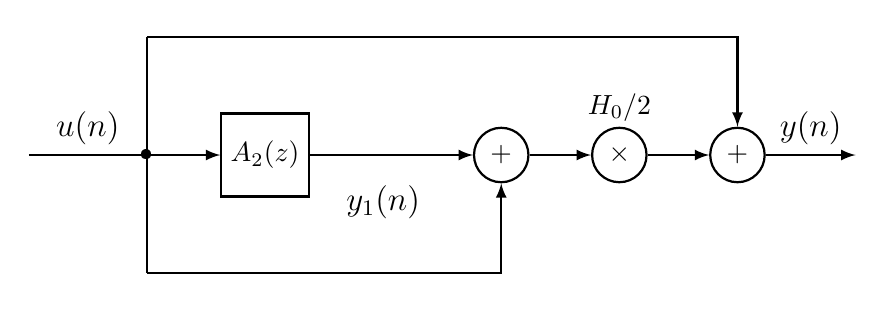
\begin{tikzpicture}[auto, thick, node distance=0.6cm, >=latex, scale = 0.75]
	\draw
	node at (2,0)[delay] (d1) {$A_2(z)$}
	node at (6,0)[sum] (s1) {$+$}
	node at (8,0)[prod](p1){$\times$} node[above of = p1]{$H_0/2$}
	node at (10,0)[sum](s2){$+$}
	node at (4,0)(n1){}
	node[below of =n1]{\large$y_1(n)$}
	;
	
	\draw[-](-2,0) -- node {\large$u(n)$}(0,0);
	\draw[->](0,0) -- node {} (d1);
	\draw[->](d1) -- node {} (s1);
	\draw[-](0,0) -- node {} (0,-2);
	\draw[->](0,-2) -| node {} (s1);
	\draw[->](s1) -- node {} (p1);
	\draw[->](p1) -- node {} (s2);
	\draw[->](s2) -- node {\large$y(n)$} (12,0);
	\draw[-](0,0) -- node {} (0,2);
	\draw[->](0,2) -| node {} (s2);
	
	\draw
	node at (0,0) {\textbullet};
	\end{tikzpicture}
\end{center}
\end{frame}

\begin{frame}
The difference equations of second-order peak filter are
\[
x(n) = u(n) - d(1 - c_{B/C})x(n - 1) + c_{B/C}x(n - 2)
\]
\[
y_1(n) = -c_{B/C}x(n) + d(1 - c_{B/C})x(n - 1) + x(n - 2)
\]
\[
y(n) = \frac{H_0}{2}[u(n) - y_1(n)] + u(n),
\]
and corresponding state and output equations are
\[
\begin{bmatrix}x(n)\\x(n-1)\end{bmatrix} = \begin{bmatrix}
-d(1-c_{B/C})&c_{B/C}\\
1&0
\end{bmatrix}
\begin{bmatrix}x(n-1)\\x(n-2)\end{bmatrix} + \begin{bmatrix}1\\0\end{bmatrix}
u(n)\]
\[
y(n) = \begin{bmatrix}\frac{H_0}{2}(c_{B/C}^2-1)d&\frac{H_0}{2}(c_{B/C}^2-1)\end{bmatrix}
\begin{bmatrix}x(n-1)\\x(n-2)\end{bmatrix} + [\frac{H_0}{2}(1+c_{B/C})+1]u(n).
\]
\end{frame}

\begin{frame}
The center frenquency parameter $d$ and the coefficient $H_0$ are given by
\[
d = -\cos(2\pi f_c/f_S)
\]
\[
V_0 = H(e^{j2\pi f_c/f_S}) = 10^{G/20}
\]
\[
H_0 = V_0 - 1.
\]
The bandwidth $f_b$ is adjusted through the parameters $c_B$ and $c_C$ for boost and cut given by
\[
c_B = \frac{\tan(\pi f_b/f_S) - 1}{\tan(\pi f_b/f_S) + 1}
\]
\[
c_C = \frac{\tan(\pi f_b/f_S) - V_0}{\tan(\pi f_b/f_S) + V_0}.
\]
\end{frame}
\begin{frame}[fragile]
Matlab code:
\begin{lstlisting}
function y = peakfiltunit(audio, para)
% Applies a peak filter to the input signal.
% para(1) is the normalized center frequency in (0,1), i.e. 2*fc/fs.
% para(2) is the normalized bandwidth in (0,1), i.e. 2*fb/fs.
% prar(3) is the gain in dB.
V0 = 10^(para(3)/20); H0 = V0 - 1;
if para(3) >= 0
    c = (tan(pi* para(2)/2)-1) / (tan(pi* para(2)/2)+1);     % boost
else
    c = (tan(pi* para(2)/2)-V0) / (tan(pi* para(2)/2)+V0);   % cut
end;
d = -cos(pi*para(1));
x = [0; 0];
x_1 = 0;
A = [-d*(1-c), c; 1, 0];
B = [1; 0];
\end{lstlisting}
\end{frame}
\begin{frame}[fragile]
\begin{lstlisting}
C = [H0/2*(c^2-1)*d, H0/2*(c^2-1)];
D = [H0/2*(1+c) + 1];
for n=1:length(audio)
    x_1 = A * x + B * audio(n);
    y(n) = C * x + D * audio(n);
    x = x_1;
end
\end{lstlisting}
\end{frame}


\end{document}